\documentclass[./einleitung.tex]{subfiles}
\usepackage{glossaries}
\normalsize

\begin{doccomment}
    \section{Die Nutzung des \acrshort{lsp}}
    \subsection{Installationsmöglichkeiten}
    Der \acrshort{lsp}-Server benötigt keine zusätzlichen Strukturen und kann direkt als Datei ausgeführt werden.
    Deshalb ist die normale Vorgehensweise das Abelgen des \acrshort{lsp}-Servers in einem Zentralen Server und das Hinzufügen des Pfades zu dem Umgebungsvariablen.
    Im Beispiel wurde die Datei zu `dmflsp' umbennant, damit der Name genauert das Programm beschreibt und nicht mit anderen \acrshort{lsp}-Server kollidieren kann.
    \begin{figure}
        \centering
        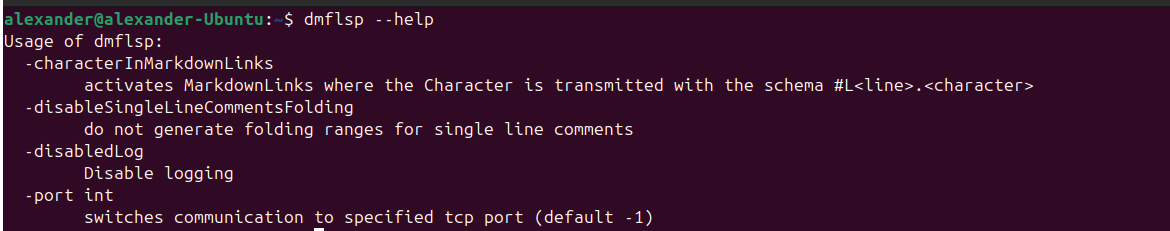
\includegraphics[width=\linewidth]{bilder/screenshot-lsp-help}
        \caption{Aufruf des \acrshort{cli} des \acrshort{lsp}-Servers}
        \label{fig:screenshot-lsp-help}
    \end{figure}
    Es gibt Editoren die eine native Anbindung eines \acrshort{lsp}-Servers ermöglichen.
        {\footnotesize TODO Zed Besspiel }
    \subsubsec{Intellij}
    Intellij unterstützt nur wenige \acrshort{lsp}-Funktionen ohne zusätzliche Plugins.
    Mit von `lsp4ij' können \acrshort{lsp}-Server direkt in der Oberfläche konfiguriert werden.
    \begin{figure}
        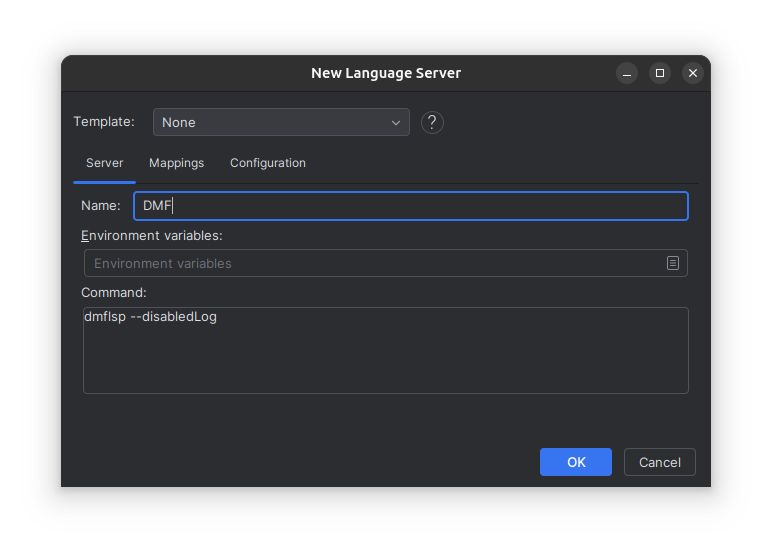
\includegraphics[width=\linewidth / 2]{bilder/screenshot-add-lsp-lsp4ij}
        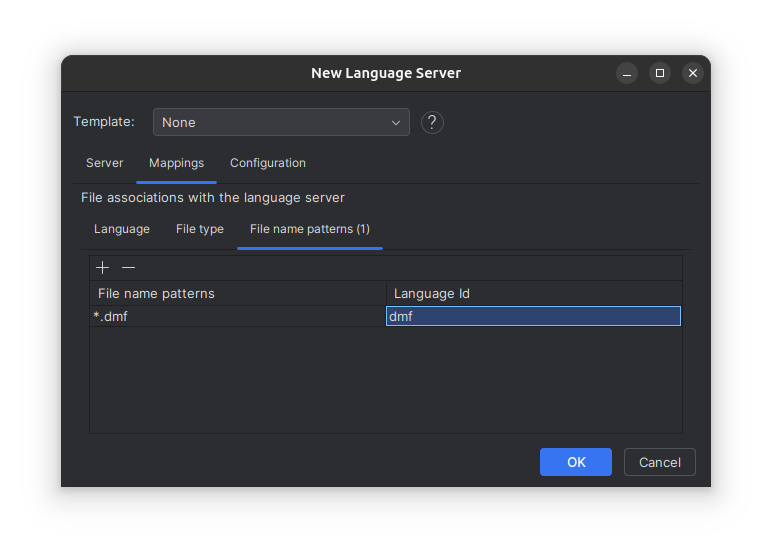
\includegraphics[width=\linewidth / 2]{bilder/screenshot-file-mapping}
        \caption{lsp4ij Konfiguration}
        \label{fig:screenshot-add-lsp-lsp4ij}
    \end{figure}
    Um diese Konfiguration automatisch anzulegen und den Dateien ein passendes Icon zu geben, kann das Intellij-Plugin für das \acrshort{dmf} verwendet werden.
    Es enthält die verschiedenen Versionen des Servers und kann sie automatisch an die Konfigurierte
\end{doccomment}